\begin{figure}[H] 
    \centering
    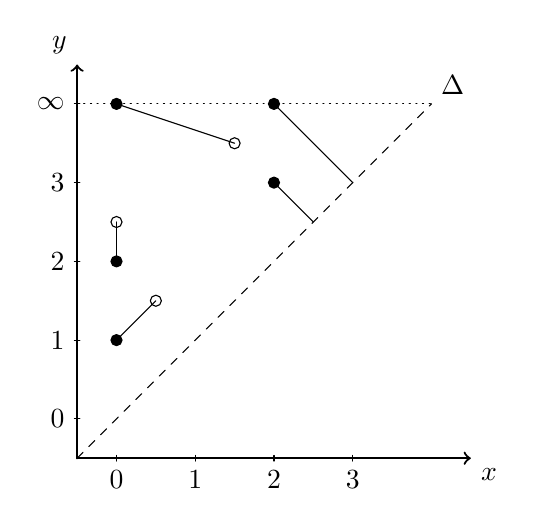
\begin{tikzpicture}[line cap=round, line join=round, x=1cm, y=1cm]
        
        \draw[thick,->] (0,0) -- (5,0) node[anchor=north west] {$x$};
        \draw[thick,->] (0,0) -- (0,5) node[anchor=south east] {$y$};
        \draw[dashed] (0,0) -- (4.5,4.5) node[above right] {$\Delta$};
        \draw[dotted] (0,4.5) -- (4.5,4.5);

        \draw (0.5 cm,1pt) -- (0.5 cm,-1pt) node[anchor=north] {0};
        \draw (1.5 cm,1pt) -- (1.5 cm,-1pt) node[anchor=north] {1};
        \draw (2.5 cm,1pt) -- (2.5 cm,-1pt) node[anchor=north] {2};
        \draw (3.5 cm,1pt) -- (3.5 cm,-1pt) node[anchor=north] {3};

        \draw (1pt,0.5 cm) -- (-1pt,0.5 cm) node[anchor=east] {0};
        \draw (1pt,1.5 cm) -- (-1pt,1.5 cm) node[anchor=east] {1};
        \draw (1pt,2.5 cm) -- (-1pt,2.5 cm) node[anchor=east] {2};
        \draw (1pt,3.5 cm) -- (-1pt,3.5 cm) node[anchor=east] {3};

        \draw (1pt,4.5 cm) -- (-1pt,4.5 cm) node[anchor=east] {$\infty$};

        \draw[fill=black] (0.5, 1.5) circle (2pt); 
        \draw[fill=black] (0.5, 2.5) circle (2pt); 
        \draw[fill=black] (0.5, 4.5) circle (2pt); 

        \draw[fill=black] (2.5, 3.5) circle (2pt); 
        \draw[fill=black] (2.5, 4.5) circle (2pt);
        
        \draw[] (1, 2) circle (2pt);
        \draw[] (0.5, 3) circle (2pt);
        \draw[] (2, 4) circle (2pt);

        \draw (0.5, 3) -- (0.5, 2.5);
        \draw (1, 2) -- (0.5, 1.5);
        \draw (0.5, 4.5) -- (2, 4);
        \draw (2.5, 4.5) -- (3.5, 3.5);
        \draw (2.5, 3.5) -- (3, 3);
        
    \end{tikzpicture}
    \caption{Wasserstein distance between two persistence diagrams.}
    \label{fig:bottleneck}
\end{figure}